\RequirePackage{snapshot}
\documentclass[a4paper,oneside]{alpenthesis/alpenthesis}
% <<< Preamble
\hexfalse
\paperfalse
%https://tex.stackexchange.com/a/210456/131649
\renewcommand\partnumberlinebox[2]{#2\hspace{2em}}
\usetikzlibrary{positioning}
\usepackage{multirow,array}
\tcbuselibrary{breakable}
\tcbset{shield externalize}
\makeindex
% >>>
\begin{document}
\begin{titlingpage} % <<<
    \fullhexpage{q1}{q0}
    \flushright\sffamily

    \vspace*{5em}
    \Huge\bfseries{Red Pitaya}\\[1ex]
    \Large\mdseries{Thesis}\\[3ex]

    \normalsize\mdseries
    
    \vfill
    Raphael Frey\\
    Noah H\"usser\\[3ex]

    \vspace{5em}

    \today\\
    Version 0.0.1
\end{titlingpage} % >>>

\frontmatter % <<<
% https://en.wikipedia.org/wiki/Edition_notice
\tableofcontents*
\clearpage
\listoffigures*
\clearpage
\listoftables*
\clearpage
\listoflistings
\clearpage
% >>>

\mainmatter

\chapter{Introduction} % <<< ------------------------------------------------- %
\label{ch:intro}
% ---------------------------------------------------------------------------- %

% ==============================================================================
%
%                           I N T R O D U C T I O N
%
% ==============================================================================
\chapter*{Introduction} % ---------------------------------------------------- %
\label{ch:intro}
\addcontentsline{toc}{chapter}{\nameref{ch:intro}}
% ---------------------------------------------------------------------------- %

Electronic measuring equipment has historically tended to be very pricey, with
specialized appliances  sometimes costing  as much as  a middle-class  car, or
even more. While high-performance  solutions are unlikely to  be replaced with
something radically  different in  the foreseeable future,  modern, affordable
FPGAs  are  a  viable  alternative  in many  use  cases  nowadays. By  keeping
performance requirements within reasonable bounds and pairing the FPGA with an
appropriate  front-end, sufficient  performance for  many applications  can be
achieved  at a  very competitive  price point.   Additionally, an  FPGA offers
vastly  superior flexibility  over the  fixed silicon  of conventional  signal
processing chips,  since its hardware  capabilities can be altered  even after
deployment.

A suitable front-end for an FPGA usually comprises dedicated ADCs and DACs and
analog  filters. Along with  FPGA chips  themselves,  ADC and  DAC chips  have
become much more economical in recent  years, resulting in a product which may
cost  as little  as  a few  hundred  Swiss  Francs and  which  can replace  an
apparatus several times as expensive.

This project  aims to  equip such an  FPGA board with  logic that  can record,
filter  and store  electrical signals  with  adjustable sampling  rates up  to
\SI{125}{\mega\hertz}.   To  complement  the hardware  subsystem,  a  software
component is provided, consisting of two applications: One runs on an embedded
GNU/Linux on the board itself, while  the other runs on a user's computer. The
application on the  board (the \emph{server}) is  responsible for transmitting
the recorded data over a network connection, while the software running on the
user's  computer  (the oscilloscope,  or  \emph{scope}  for short)  serves  to
visualize and  process the  measurement results. This  concept is  depicted in
Figure~\ref{fig:intro:system_overview}.

\makeatletter
\renewcommand{\thefigure}{\@arabic\c@figure}
\makeatother
\begin{figure}
    \centering
    \tikzsetnextfilename{intro-system-overview}
\begin{tikzpicture}[
    rounded corners=1mm,
    node distance=5mm,
    fpgaComponent/.style={
        draw,
        minimum height=12ex,
        fill=q4,
    },
    SoCComponent/.style={
        minimum height=8ex,
        minimum width=6em,
        fill=ct2,
        draw=sqC,
        text=br2,
        font=\bfseries,
    },
]
    \small
    \sffamily

    \node[SoCComponent] at (0,0) (fpga) {FPGA};
    \node[SoCComponent,right=of fpga] (server) {Server};

    \begin{scope}[on background layer]
        \node[
            draw=black,
            fit=(fpga) (server),
            inner sep=2mm,
            align=left,
            text height=11ex,
            minimum height=16ex,
            fill=br1,
            text=black,
            font=\bfseries,
        ] (board) {Board};
    \end{scope}

    \node[
        right=10mm of board,
        minimum width=12ex,
        minimum height=8ex,
        fill=ct2,
        align=center,
        text=br2,
    ] (pcmonitor) {\bfseries Scope\\\\};

    \begin{scope}[on background layer]
        \node[
            draw=black,
            fit=(pcmonitor),
            minimum height=8ex,
            fill=black!60!white,
        ] (pcmonitorframe) {};
    \end{scope}

    \fill[br2] ($(pcmonitorframe.south) + (-1ex,0)$) --+ (0,-1ex) --+ (2ex,-1ex) --+ (2ex,0) -- cycle;
    \draw ($(pcmonitorframe.south) + (-1ex,0)$) --+ (0,-1ex);
    \draw ($(pcmonitorframe.south) + (1ex,0)$)--+ (0,-1ex);
    \draw ($(pcmonitorframe.south) + (1ex,0)$)--+ (0,-1ex);
    \draw[fill=br2] ($(pcmonitorframe.south) + (-6ex,-1ex)$) rectangle
          ($(pcmonitorframe.south) + (+6ex,-3ex)$);

    \draw[thick,-latex] (-18.0mm,0mm) -- ($(board.west) + (-1mm,0mm)$);
    \draw[thick,-latex] ($(board.east) + (1mm,0mm)$) -- ($(pcmonitorframe.west) + (-1mm,0mm)$);
    \draw[thick,-latex] ($(fpga.east) + (0.5mm,0mm)$) -- ($(server.west) + (-0.5mm,0mm)$);

    \begin{axis}[
        anchor=east,
        at={(-20mm,0mm)},
        width=20mm,
        height=10mm,
        axis line style={draw=none},
        tick style={draw=none},
        grid=none,
        ticks = none,
        xmin=0,
        xmax=360,
        ymin=-1.1,
        ymax=1.1,
        samples=500,
    ]
        \addplot[line cap=round,very thick,q1,domain=0:360,-]{sin(x)};
    \end{axis}

    \begin{axis}[
        anchor=south,
        yshift=1mm,
        at={(pcmonitor.south)},
        width=12mm,
        height=6mm,
        axis line style={draw=none},
        tick style={draw=none},
        grid=none,
        ticks = none,
        xmin=0,
        xmax=360,
        ymin=-1.3,
        ymax=1.3,
        samples=500,
    ]
        \addplot[very thick,q4,domain=0:360]{sin(x)};
    \end{axis}

    \node[font=\bfseries\footnotesize,text=black] at (-29mm,-8.95mm) {Signal};
\end{tikzpicture}

    \caption[System Overview]{%
        An overview of the main system components.  An analog signal (left) is
        measured, the data  goes into the server  and is  then transmitted via
        network to a computer running the scope.%
    }
    \label{fig:intro:system_overview}
\end{figure}
\makeatletter
\renewcommand{\thefigure}{\thechapter.\@arabic\c@figure}
\makeatother

The  objective  of  this  project  is   to  provide  a  device  which  enables
students and hobbyists  to analyze signals encompassing the  region from audio
frequencies  to the  low megahertz  range. Compared to  the frequencies  which
modern hardware  can handle  (dozens to hundreds  of megahertz),  the sampling
rates required to process such signals  can be kept within the limits suitable
for an FPGA.

A RedPitaya  STEMlab 125-14 board  is used as  the basis for  the hardware. It
easily offers  sufficient performance  to process the  signals in  the desired
range, having an  ADC which provides a \SI{14}{\bit}  signal at \SI{125}{\MHz}
on two channels.   Indeed, downsampling this signal is  \emph{necessary} if it
is  to be  transmitted over  a  network connection,  since its  data rate  far
exceeds the available bandwidth.

Thus, two primary objectives can be defined:
\begin{enumerate}\tightlist
    \item
        The signal coming out of the ADC must be decimated.
    \item
        The resulting data stream must be visualized for the end user.
\end{enumerate}

Downsampling the  data provided by the  ADC is performed on  the FPGA. Because
downsampling introduces  unwanted frequencies  into the signal's  spectrum, it
needs  to be  processed  by filters  which  attenuate those  components. While
the  STEMlab  offers  some  limited  capability in  this  area  in  its  stock
configuration,  this was  deemed insufficient  and has  been improved  in this
project. Several  filter  chains are  implemented  to  allow decimation  rates
between \num{5}  and \num{2500},  corresponding to output  frequencies between
\SI{25}{\MHz}  and \SI{50}{\kHz},  respectively. The  server application  then
transmits the filtered data stream over Ethernet to a client.

The filter chains have achieved a  signal-to-noise ratio of up to \SI{84}{\dB}
in tests,  depending on  the chosen  chain and  input frequency. Additionally,
the  \SI{14}{\bit}  signal from  the  ADC  is  improved by  \SI{1.2}{\bit}  to
\SI{1.8}{\bit}, again depending on  the chain. Passband shapes show negligible
droop, and stopband aliasing is \SI{60}{\dB}.

Cost-effective FPGA  boards like the  STEMlab usually come without  a physical
user interface  with displays and  buttons. This keeps the device  compact and
its cost  low.  Since fast  personal computers  are ubiquitous these  days, it
seems obvious  to exploit that and  run an oscilloscope application  on such a
device. Due to  the fragmentation of  the modern computing world  into various
ecosystems (Windows, GNU/Linux, macOS, Android, \ldots), web technologies form
the foundation of  the scope; the application can be  accessed from any modern
browser. This makes life easier both for the developers and for the end users.

\paragraph{This      document      is      split      into      four      main
parts:} Part~\ref{part:project_report},    contains   the    primary   project
report. Part~\ref{part:Developer_Guide}   is   the    developer   guide,   and
begins   on  page~\pageref{part:Developer_Guide}. A   short   user  guide   is
provided  in  Part~\ref{part:User_Guide}  from  page~\pageref{part:User_Guide}
onwards. Appendices   are   located   on   page~\pageref{ch:app:fdesign}   and
onwards.
%Depending  on  the  report version,  Appendix~\ref{ch:app:media}  may
%contain a copy of the project repository.

The   project  report   covers  information   relevant  to   the  design   and
implementation of the final product. Its first chapter starts on presents some
relevant theoretical background on digital signal processing, with an emphasis
on digital  filtes  and CIC  filters in particular. The next  chapter outlines
the  process leading  to  the concept  for  our product,  and  compares a  few
alternative choices against it, beginning on page~\pageref{ch:mission}.

The    design   and    implementation    of   the    product   is    detailled
in     Chapters~\ref{ch:filter_design},     \ref{ch:fpga},     \ref{ch:server}
and~\ref{ch:graphical_front_end}. Chapter~\ref{ch:filter_design} documents the
filter  design;  both  requirements   and  specifications  are  documented. An
overview  of  the  FPGA  implementation  is  given  in  Chapter~\ref{ch:fpga},
highlighting some key points  which proved challenging during development. The
transmission   of   data   between   STEMlab  and   client   is   handled   by
a   server   application,  documented   in   Chapter~\ref{ch:server}. Finally,
the    concepts   and    design   choices    underpinning   the    scope   are
explained   in    Chapter~\ref{ch:graphical_front_end}. The   chapters   begin
on  pages~\pageref{ch:filter_design},  \pageref{ch:fpga},  \pageref{ch:server}
and~\pageref{ch:graphical_front_end}, respectively.

The  product's  performance  is assessed  in  \emph{\nameref{ch:verification}}
from page~\pageref{ch:verification}  onwards, and Chapter~\ref{ch:conclusions}
contains some  concluding remarks  on the overall  result and  possible future
steps.

The Developer and  User Guides are mostly  self-contained. The Developer Guide
is  intended for  people who  wish to  use  our product,  or parts  of it,  to
implement a system of their own. The  User Guide is intended for end-users who
wish to perform measurements with our product.

\enlargethispage{6ex}
\vspace{1ex}
\noindent All  components specifically developed  for this project  fall under
the MIT license, a copy of which is located in Appendix~\ref{ch:app:licenses}.

%^^A vim: foldenable foldcolumn=4 foldmethod=marker foldmarker=<<<,>>>


\begin{itemize}\firmlist
    \item Rationale (Why?)
    \item What is the general approach to solve this problem?
    \item What has been done so far?
    \item Results of previous work
    \item What are we going to do?
    \item What are the contents of this report?
\end{itemize}

\cite{1163535}

% >>>

\part{System Overview} % <<< ------------------------------------------------- %
\label{part:System_Overview}
% ---------------------------------------------------------------------------- %

Fundamental question  to answer in  this part:  \emph{What is our  system, and
what is it good for?}

This information could also go into \emph{Introduction}?

Provide supplementary theoretical background as needed.


\chapter{Analog-to-Digital Data Acquisition} % <<< --------------------------- %
\label{ch:analog-to-digital_data_aquisition}
% ---------------------------------------------------------------------------- %

\begin{itemize}
    \item
    Generic Chapter on some of the basic principles of AD data processing
    \item
    Sampling:
        \begin{itemize}
            \item
            \index{Sampling} in time domain: Multiplication with dirac pulse sequence
            \item
            Frequency doman: Convolution of signal spectrum and dirac pulse spectrum
            \item
            ``What is spectrum of dirac pulse sequence?'' (dirac pulse sequence)
            \item
            Consequently: \index{Spectrum} of sampled signal is repeated for each dirac pulse in the spectrum
            \item
            \textbf{Make sure to get distances between pulses as well as heights correct!}
            \item
            \index{Aliasing}
            \item
            LP-Filtering (Anti-Aliasing Filter)
            \item
            Potentially mention reconstruction
        \end{itemize}
    \item 
    Very brief mention of aliasing, low-pass filtering and all that
    \item
    Oversampling and Downsampling
    \item
    Oversampling: Explain advantage w/r to SNR
    \item
    Fancy graphics from Mr. Gut
    \item
    How does the Red Pitaya fit into this?
    \item
    CIC and FIR filters:
        \begin{itemize}
            \item
            Overview (emphasis on CIC)
            \item
            Where to use which, and why?
            \item
            Table/Matrix with advantages and drawbacks for each
            \item
            How does this translate to our system/Why is this important for us?
        \end{itemize}
\end{itemize}

Explain processing chain (do we even have an analog LP filter here?)

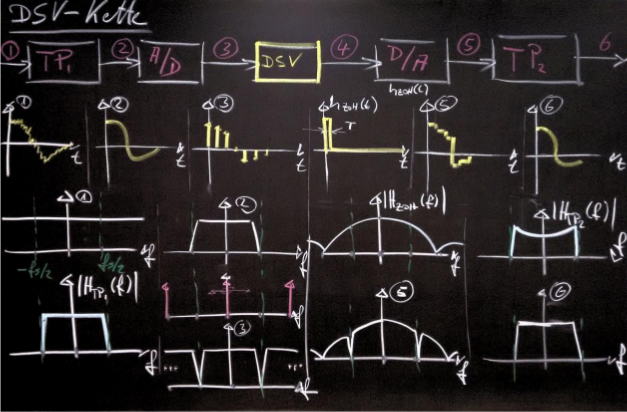
\includegraphics[width=0.75\textwidth]{images/dsvChain}

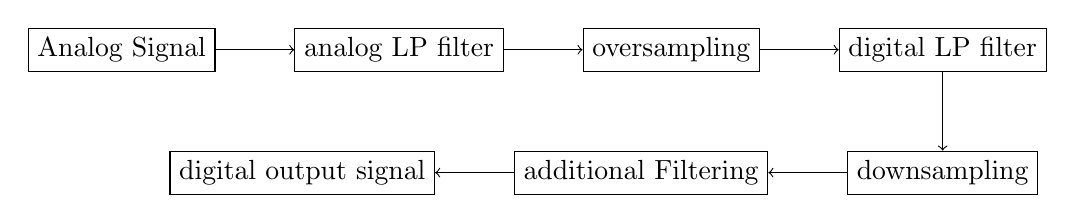
\begin{tikzpicture}[
        every node/.style={draw}
    ]
    \node (analog) at (0,0) {Analog Signal};
    \node[right=of analog] (lpf) {analog LP filter};
    \node[right=of lpf] (sampling1) {oversampling};
    \node[right=of sampling1] (lpf2) {digital LP filter};
    \node[below=of lpf2] (downsampling) {downsampling};
    \node[left=of downsampling] (addf) {additional Filtering};
    \node[left=of addf] (digital) {digital output signal};

    \draw[->] (analog) -- (lpf);
    \draw[->] (lpf) -- (sampling1);
    \draw[->] (sampling1) -- (lpf2);
    \draw[->] (lpf2) -- (downsampling);
    \draw[->] (downsampling) -- (addf);
    \draw[->] (addf) -- (digital);
\end{tikzpicture}

% >>>

\chapter{The Red Pitaya Platform} % <<< -------------------------------------- %
\label{ch:the_red_pitaya_platform}
% ---------------------------------------------------------------------------- %
\section{General Information}
General Info about Red Pitaya Project:
\begin{itemize}\firmlist
    \item How is the PITA project structured? (logically, license-wise, philosophically)
    \item Why do we care about this?
    \item Replacement for scopes (motivation: Why would one use the PITA?)
\end{itemize}
\subsection{FPGA}
\subsection{Linux}

\section{Performance and Possible Improvements}
\begin{itemize}
    \item
    What is the stock solution for downsampling and such? Performance?
    \item
    Results of Previous Work
    \item
    Consequences for us: Possible paths forward
    \item
    System Analysis
    \item 
    Decision Matrix \& Decision
    \item
    pgfplots: Ternary diagram?
\end{itemize}

% >>>

% >>>

\part{Implementation} % <<< -------------------------------------------------- %
\label{part:Implementation}
% ---------------------------------------------------------------------------- %
Implementation can be read independently of previous part, but there should be
a  red thread  from decision  to \index{implementation}. Deals  primarily with
design decisions.

Present a diagram with all  system components. Then document the components in
their respective chapters and sections.

\chapter{Data Acquisition System}
\label{ch:data_acquisition_system}
\section{FPGA}
\section{Kernel Module}

\chapter{Filters} % <<< ------------------------------------------------------ %
\label{ch:filters}
% ---------------------------------------------------------------------------- %

% >>>

\chapter{Server} % <<< ------------------------------------------------------- %
\label{ch:server}
% ---------------------------------------------------------------------------- %

% >>>

\chapter{Graphical Front End} % <<< ------------------------------------------ %
\label{ch:graphical_front_end}

%\section{Scope}

\begin{frame}
    \frametitle{Demo}

    \centering
    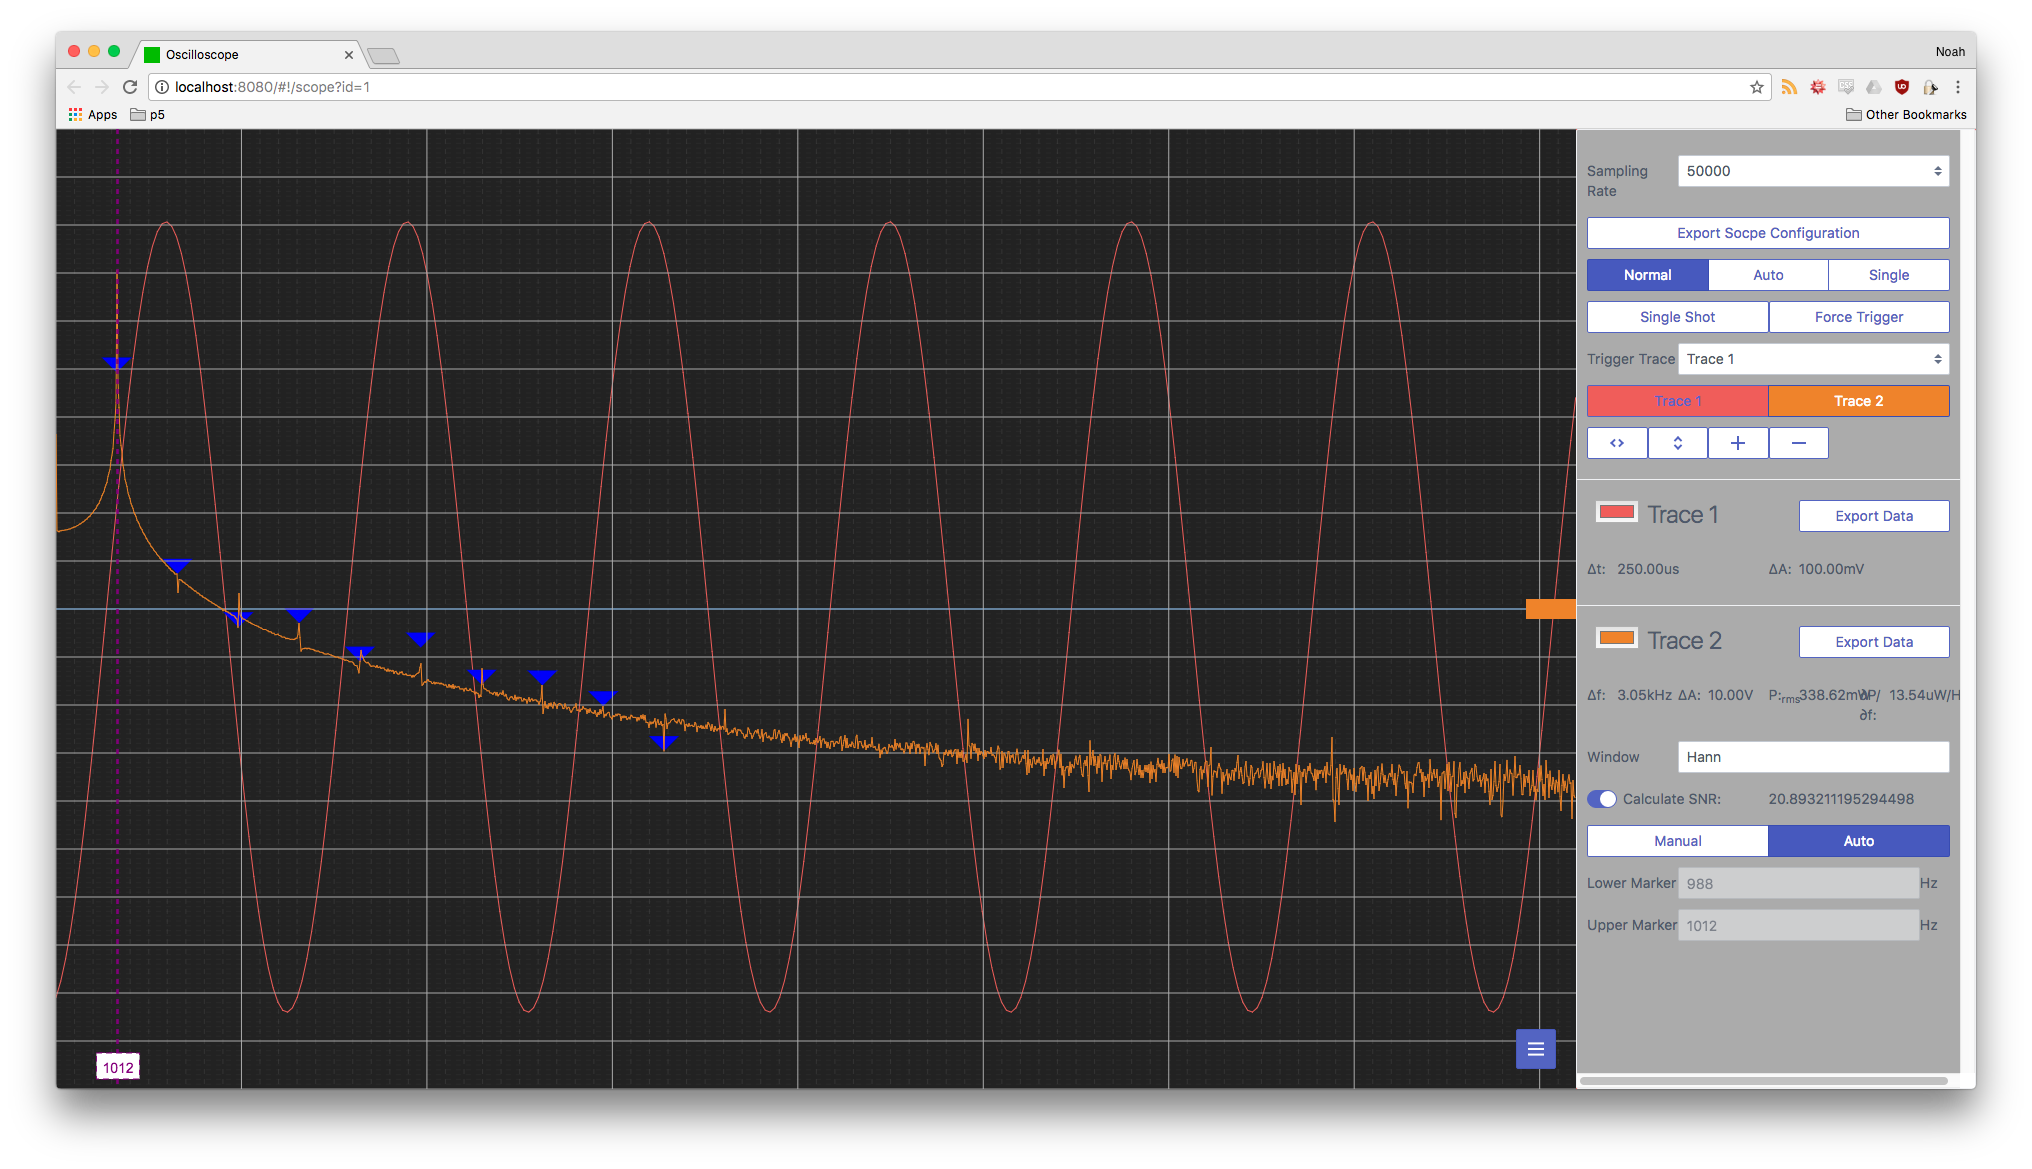
\includegraphics[width=1\textwidth]{images/scope}
\end{frame}

\begin{frame}
    \frametitle{Technologies used}

    \centering
    \begin{tikzpicture}
        \node at (0,0) {
\includegraphics[width=2cm]{images/logos/JS.jpeg}};
        \node at (4,-1) {
\includegraphics[width=2cm]{images/logos/webgl.jpeg}};
        \node at (0,-4) {
\includegraphics[width=2cm]{images/logos/uws.jpeg}};
        \node at (4,-4) {
\includegraphics[width=2cm]{images/logos/mithril.png}};
    \end{tikzpicture}
\end{frame}


% >>>

% >>>

\part{Developer Guide} % <<< -------------------------------------------------- %
\label{part:Developer_Guide}
% ---------------------------------------------------------------------------- %
Documentation for a person who wishes to utilize our system in their work and/or
improve upon it?

Make sure  to distinguish  between \emph{Implementation} and  this part. Lines
seem a bit blurry to me (R.F.) at the moment (\today).

\chapter{Project Structure} % <<< -------------------------------------------- %
\label{ch:Project_Structure}
% ---------------------------------------------------------------------------- %
Structure of the repository. What can be found where, and what to do with it?

% >>>

\chapter{IP Core} % <<< ------------------------------------------------------ %
\label{ch:IP_Core}
% ---------------------------------------------------------------------------- %
Documentation of our FPGA Project (structure, interfaces, registers \ldots)

% >>>

\chapter{Linux} % <<< -------------------------------------------------------- %
\label{ch:Linux}
% ---------------------------------------------------------------------------- %

Kernel module, server

% >>>

\chapter{Tool Chain} % <<< --------------------------------------------------- %
\label{ch:Tool_Chain}
% ---------------------------------------------------------------------------- %
Vivado, Build Box, ARM Linux, TCL, Makefiles, Libs for building server application

% >>>

% >>>

\part{User Guide} % <<< ------------------------------------------------------ %
\label{part:User_Guide}
% ---------------------------------------------------------------------------- %
Documentation  for the  end user. Primarily  concerned with  the \index{scope}
front-end.

% >>>

\cleardoublepage % <<< ---------------------------------------------APPENDICES %
\begin{titlingpage*}
    \fullhexpage{da2}{ct4}
    \begin{vplace}
        \flushright\Huge\bfseries\sffamily\appendixpagename
    \end{vplace}
\end{titlingpage*}
\appendix
\chapterstyle{alpenappendix}
% ---------------------------------------------------------------------------- %

% Matlab-prettifier: Uses the lstlisting counter
% Minted: Uses the listing counter

\chapter{Code Listings}
\label{ch:Code_Listings}

Shell commands can be type thusly:
\begin{commandshell}
    user:> if [ -f "${myfile}" ];then echo "${myfile} exists!"
\end{commandshell}

\section{Makefile}
\begin{tcolorbox}[
        breakable,
        title={
            \refstepcounter{listing}
            Listing \thelisting: Makefile Code
            \label{lst:makefile}
            \addcontentsline{lol}{listing}{\protect\numberline{\thelisting}Makefile Code}
        }
    ]
    \inputminted{makefile}{code/Makefile}
\end{tcolorbox}

\section{Verilog}
\begin{tcolorbox}[
        breakable,
        width=1.2\textwidth,
        title={
            \refstepcounter{listing}
            Listing \thelisting: Verilog Code
            \label{lst:makefile}
            \addcontentsline{lol}{listing}{\protect\numberline{\thelisting}Verilog Code}
        }
    ]
\inputminted{verilog}{./code/axi_axis_reader.v}
\end{tcolorbox}

\section{VHDL}
\inputminted{vhdl}{./code/comparator.vhd}

\section{TCL}
\inputminted{tcl}{./code/create_cores.tcl}

\begin{listing}
    \begin{minted}[autogobble]{vhdl}
        entity comparator is
            generic (
                Width : integer := 14
            );
            port (
                AxDI : in unsigned(Width - 1 downto 0);
                BxDI : in unsigned(Width - 1 downto 0);
                GreaterxSO : out std_logic;
                EqualxSO : out std_logic;
                LowerxSO : out std_logic
            );
        end comparator;
    \end{minted}
    \caption{Comparator}
    \label{lst:vhdl:comparator}
\end{listing}

\section{Matlab}
Here, we shall also demonstrate breaking a code file into multiple segments
to comment on its contents.

We start with the header:
\begin{tcolorbox}[
        skin = octoboxfirst,
        title={
            \refstepcounter{listing}
            Listing \thelisting: Matlab Code
            \label{lst:makefile}
            \addcontentsline{lol}{listing}{\protect\numberline{\thelisting}Matlab Code}
        }
    ]
    \inputminted[
        linenos,
        numbersep=4pt,
        style=solarizedlight,
        firstline=1,
        lastline=12,
    ]{matlab}{./code/filterChainDesigns.m}
\end{tcolorbox}
In the next box, we start where we  left off previously, and we pack some more
header information into our listing:
\begin{tcolorbox}[
        skin = octoboxmiddle,
    ]
    \inputminted[
        linenos,
        numbersep=4pt,
        style=solarizedlight,
        firstnumber=last,
        firstline=13,
        lastline=26,
    ]{matlab}{./code/filterChainDesigns.m}
\end{tcolorbox}

Then we describe the target for the FIR filter:
\begin{tcolorbox}[
        skin = octoboxmiddle,
    ]
    \inputminted[
        linenos,
        numbersep=4pt,
        style=solarizedlight,
        firstnumber=29,
        firstline=29,
        lastline=40,
    ]{matlab}{./code/filterChainDesigns.m}
\end{tcolorbox}

After which we start the sript proper by setting up the iteration parameters:
\begin{tcolorbox}[
        skin = octoboxmiddle,
    ]
    \inputminted[
        linenos,
        numbersep=4pt,
        style=solarizedlight,
        firstnumber=43,
        firstline=43,
        lastline=64,
    ]{matlab}{./code/filterChainDesigns.m}
\end{tcolorbox}

We define some data structures to contain the filter objects for further processing:
\begin{tcolorbox}[
        skin = octoboxmiddle,
    ]
    \inputminted[
        linenos,
        numbersep=4pt,
        style=solarizedlight,
        firstnumber=66,
        firstline=66,
        lastline=78,
    ]{matlab}{./code/filterChainDesigns.m}
\end{tcolorbox}

And then we iterate:
\begin{tcolorbox}[
        skin = octoboxlast,
    ]
    \inputminted[
        linenos,
        numbersep=4pt,
        style=solarizedlight,
        firstnumber=80,
        firstline=80,
        %lastline=78,
    ]{matlab}{./code/filterChainDesigns.m}
\end{tcolorbox}

% >>>

\backmatter
\bibliographystyle{IEEEtran}
\bibliography{chunks/references}
% Indexing: memman.pdf, pp. 302ff.
\printindex
\end{document}
%^^A vim: foldenable foldcolumn=4 foldmethod=marker foldmarker=<<<,>>>
